\chapter{Tổng quan}

\section{Giới thiệu về hệ thống robot tự hành thông minh và các ứng dụng}
\subsection{Giới thiệu}

Robotics đã đạt được thành tựu cực kì lớn trong công nghiệp sản xuất với robot công nghiệp như cánh tay robot (manipulator). Cánh tay robot có thể di chuyển với tốc độ và độ chính xác cao, cải thiện đáng kể năng suất và sản phẩm trong sản xuất công nghiệp.
\cite{siegwart2011introduction}

\begin{figure}[h]
    \centering
    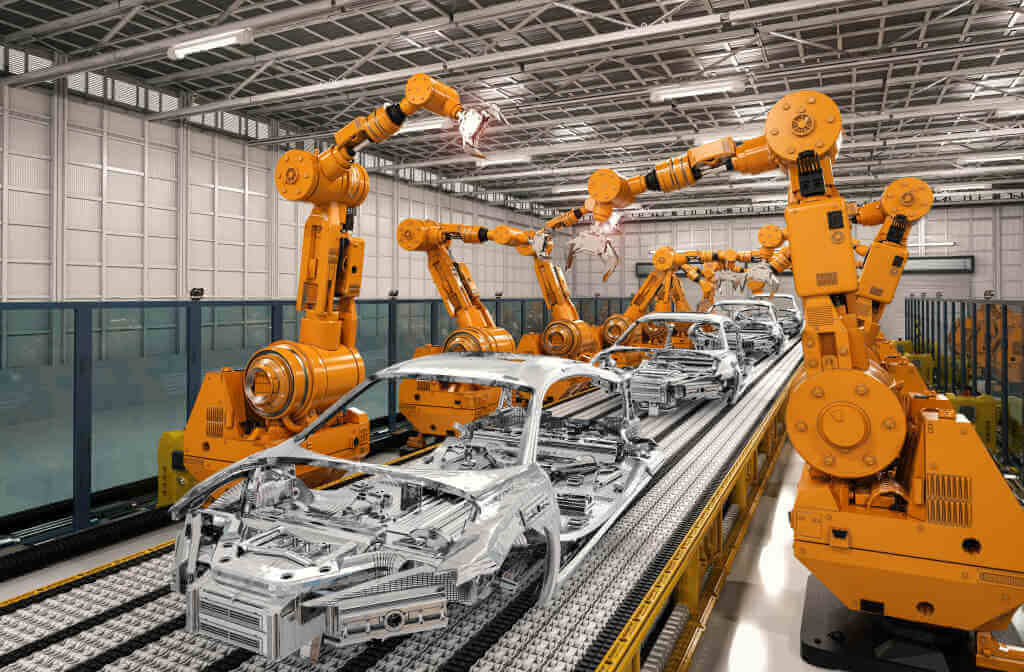
\includegraphics[width=13cm]{chapter1/figs/IndustrialRobot.jpg}
    \caption{Robot công nghiệp}
\end{figure}

Tuy vậy, hạn chế của cánh tay robot là không gian làm việc cố định và có giới hạn.

Để khắc phục hạn chế đó của cánh tay robot công nghiệp, \textit{mobile robot} hay còn gọi là robot di động ra đời. 
Ở thời điểm đầu, mobile robot chỉ có thể làm việc trong giới hạn sự kiểm soát của con người về mặt không gian và hành động. Thông qua việc điều khiển mọi hành động di chuyển của mobile robot. Ví dụ như điều khiển bằng tay thông qua bảng điều khiển, qua sóng RF... hay di chuyển bám line, đọc mã bar, mã QR. Tất cả các phương pháp đó đều khá hạn chế về không gian hoạt động cũng như yêu cầu thiết lập môi trường hết sức tốn kém, kém linh hoạt. Mỗi khi cần thực hiện một nhiệm vụ khác đều phải thiết lập lại nhà máy, không gian làm việc hết sức tốn kém.
Như vậy, làm sao để mobile robot có thể di chuyển trong môi trường thế giới thực mà không cần (hoặc ít) sự kiểm soát, điều khiển của con người để tự nó thực hiện mọi hành động đã đặt ra một số bài toán thách thức cho các nhà nghiên cứu robotics.
Từ đó, robot tự hành thông minh ra đời. 

\subsection{Robot tự hành thông minh}
Robot tự hành thông minh là loại robot di động, có thể cảm nhận, mô hình hóa môi trường xung quanh nó. Thực hiện các hành động di chuyển mà không cần sự giám sát cũng như điều khiển trực tiếp từ con người (\figurename{\ref{fig:intro}}).

\begin{figure}
	\centering
	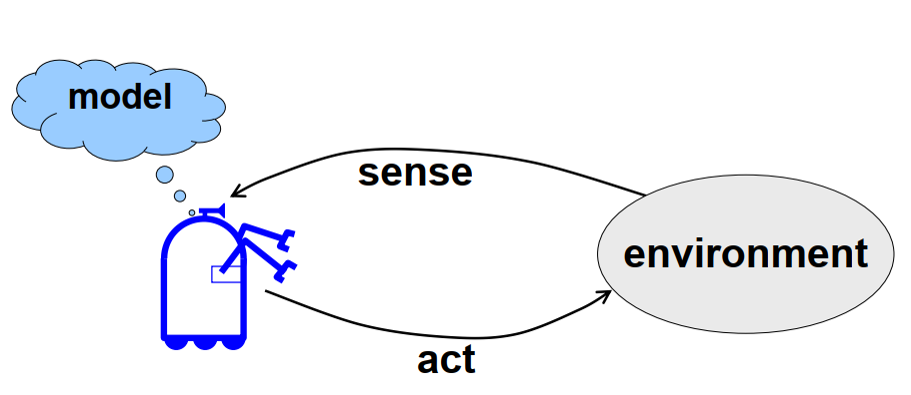
\includegraphics[width=13cm]{chapter1/figs/intro.png}
	\caption{Robot tự hành thông minh}
	\label{fig:intro}
\end{figure}

\begin{figure}
	\centering
	\subfloat[][]{
		\label{fig:ex3-a}
		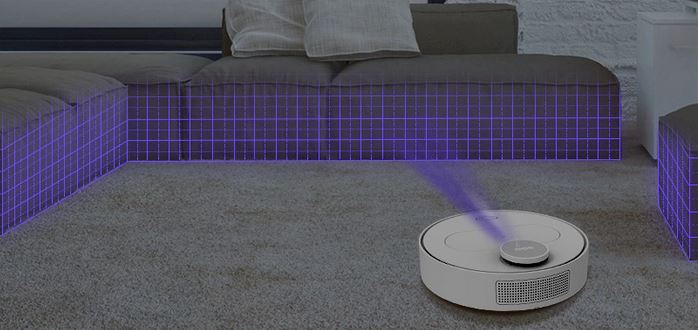
\includegraphics[width=0.4\columnwidth]{chapter1/figs/cleanerRb_2.JPG}}
	\hspace{8pt}
	\subfloat[][]{
		\label{fig:ex3-b}
		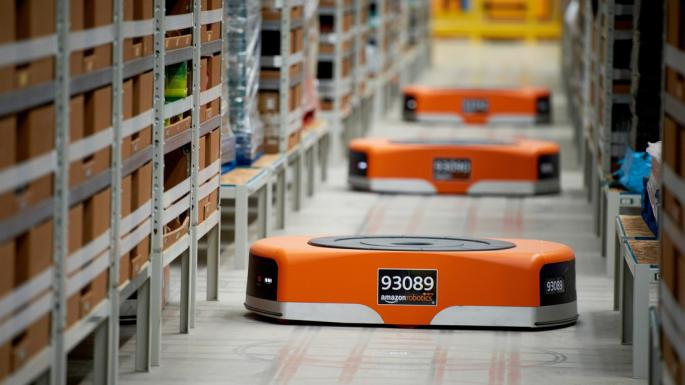
\includegraphics[width=0.4\columnwidth]{chapter1/figs/mobilerb_amazon.jpg}}\\
	\subfloat[][]{
		\label{fig:ex3-c}
		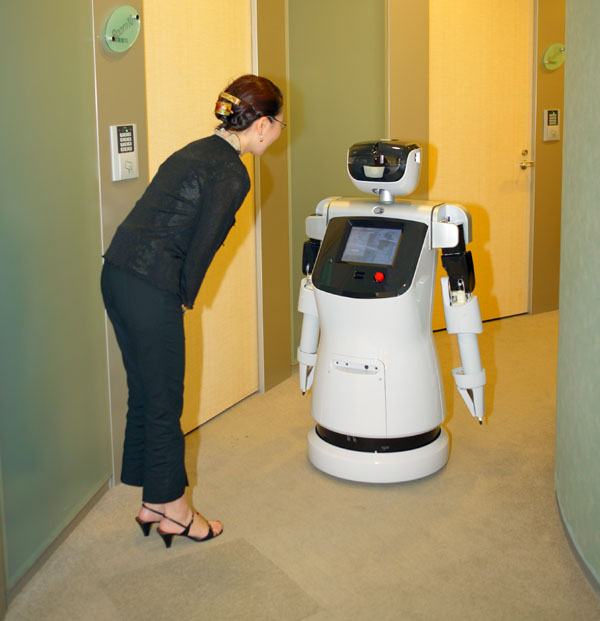
\includegraphics[width=0.4\columnwidth]{chapter1/figs/serviceRB.jpg}}
	\hspace{8pt}
	\caption[]{Một số robot tự hành:\subref{fig:ex3-a} Robot hút bụi; \subref{fig:ex3-b} Robot trong kho hàng; \subref{fig:ex3-c} Robot dịch vụ phục vụ trong khách sạn.}
	\label{fig:ex3}
\end{figure}

\subsection{Ứng dụng của robot tự hành thông minh}
Với sự thông minh và linh hoạt của của nó, Robot tự hành thông minh có rất nhiều ứng dụng, như: (\figurename{\ref{fig:applications}})

\begin{itemize}
	\item Các ứng dụng trong nhà như robot hút bụi thông minh, robot dịch vụ, robot vận chuyển trong các kho hàng...
	\item Robot thám hiểm dưới nước, trong lòng đất, trên các hành tinh khác...
	\item Robot làm việc tại các khu vực nguy hiểm như khu vực nhiễm chất phóng xạ, robot chữa cháy...
	\item Xe tự lái
\end{itemize}

\begin{figure}
	\centering
	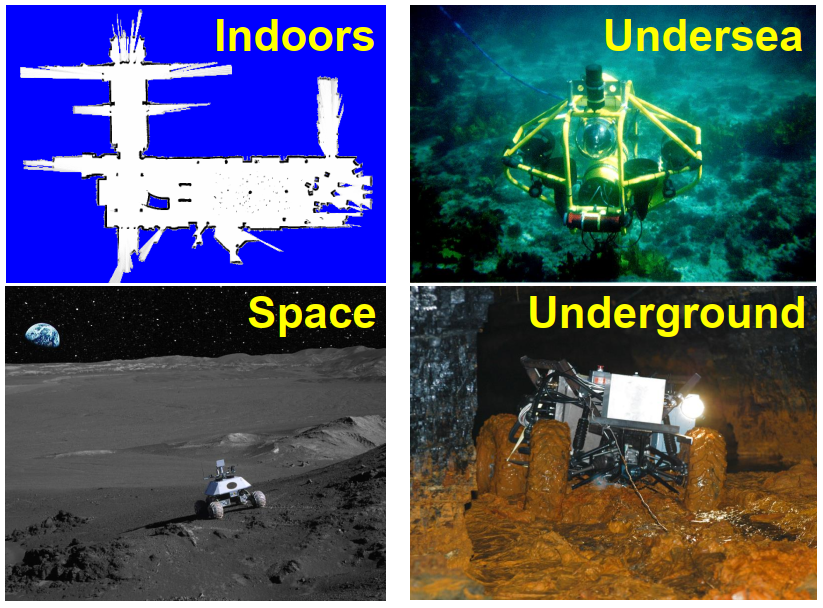
\includegraphics[width=13cm]{chapter1/figs/applications.PNG}
	\caption{Các ứng dụng của robot tự hành \cite{Burgard2010}}
	\label{fig:applications}
\end{figure}

\section{Công nghệ và bài toán cơ bản trên hệ thống robot tự hành thông minh}
\subsection{Cảm biến}
Robot tự hành thông minh cần một số loại cảm biến để có thể hiểu được môi trường, định vị và di chuyển tránh vật cản. 

Có rất nhiều loại cảm biến, để cảm nhận được đa dạng thông tin của môi trường. Có thể chia làm các nhóm như sau:
\begin{itemize}
	\item Khoảng cách 1D: Cảm biến khoảng cách hồng ngoại, siêu âm
	\item Khoảng cách 2D: Lidar
	\item Cảm biến 3D: Có nhiều loại cảm biến 3D như Intel realsense, Microsoft Kinect, Asus Xction...
	\item Ước tính trạng thái robot: GPS, IMU
	\item Cảm biến lực, momen, cảm biến chạm...
	\item Âm thanh, giọng nói như microphone, microphone array
	\item Các loại camera 2D
\end{itemize}

\begin{figure}
	\centering
	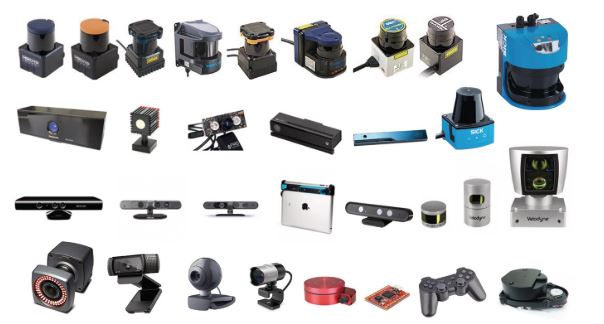
\includegraphics[width=\linewidth]{chapter1/figs/CacloaiCB.JPG}
	\caption{Một số loại cảm biến}
	\label{fig:cacLoaiCambien}
\end{figure}

\subsection{Các bài toán cơ bản trên hệ thống robot tự hành}
Định vị

Xây dựng bản đồ

Điều hướng robot

Tránh vật cản

